\section{Dirty Data Accumulation and the Cost of Deferred Cleaning}
\label{sec:eval:dynamic:dirty}

The comparison in \autoref{sec:eval:dynamic} is only meaningful if \project{}
is configured to behave as much like an in-memory system as its architecture
permits. As described earlier, we disable the write-ahead log, disable periodic
checkpointing, and size WiredTiger's cache at 800\,GiB so that the working set
never approaches the eviction thresholds. This section examines what that
configuration does to the storage engine, because the answer qualifies
every ingest and update number we report: \project{} \emph{defers} the cost of
persistence. The graph is written to disk eventually;
the configuration only controls when, and how violently.

\subsection{The knobs in play}
\label{sec:eval:dynamic:dirty:knobs}

WiredTiger governs cache pressure with a set of thresholds expressed as
percentages of the configured cache size. Two are conventional: a
\emph{target}, at which background eviction threads begin working, and a
\emph{trigger}, above which application threads are conscripted into performing
eviction on their own behalf before their operation may proceed. What makes the
system difficult to reason about is that these thresholds exist in three
parallel families, and that two of the three are \emph{derived} rather than
configured. \autoref{tab:wt-eviction-knobs} lists them for the two settings we
compare.

%%%%%%%%%%%%%%%%%%%%%%%%%%%%%%%%%%%%%%%%%%%%%%%%%%%%%%%%%%%%%%%%%%%%%%%%%%%%%%%%
\begin{table}[t]
  \centering
  \setlength{\tabcolsep}{4pt}\renewcommand{\arraystretch}{1.05}
  \small
  \begin{tabular}{l l rr rr}
  \toprule
   & & \multicolumn{2}{c}{\project{} setting} & \multicolumn{2}{c}{WiredTiger default} \\
  \cmidrule(lr){3-4}\cmidrule(lr){5-6}
  Threshold & Governs & \% & GiB & \% & GiB \\
  \midrule
  \texttt{eviction\_target}          & background, total  & 80   & 640 & 80 & 640 \\
  \texttt{eviction\_trigger}         & \textbf{app thread}, total & 95   & 760 & 95 & 760 \\
  \texttt{eviction\_dirty\_target}   & background, dirty  & 85   & 680 & 5  & 40  \\
  \texttt{eviction\_dirty\_trigger}  & \textbf{app thread}, dirty & 95   & 760 & 20 & 160 \\
  \texttt{eviction\_updates\_target}$^\dagger$  & background, updates & 42.5 & 340 & 2.5 & 20 \\
  \texttt{eviction\_updates\_trigger}$^\dagger$ & \textbf{app thread}, updates & 47.5 & 380 & 10 & 80 \\
  \bottomrule
  \end{tabular}
  \caption{WiredTiger eviction thresholds on an 800\,GiB cache. $^\dagger$The
  \emph{updates} pair is not configured by either setting: when left unset
  WiredTiger derives them as half of the corresponding dirty threshold. They are
  nevertheless the thresholds that bind in this workload. All comparisons are
  made against the byte count inflated by \texttt{cache\_overhead}, 8\% by
  default.}
  \label{tab:wt-eviction-knobs}
\end{table}
%%%%%%%%%%%%%%%%%%%%%%%%%%%%%%%%%%%%%%%%%%%%%%%%%%%%%%%%%%%%%%%%%%%%%%%%%%%%%%%%

Three properties of this scheme matter for our results.

\textbf{The thresholds are proportions of the cache, not absolute quantities.}
A cache sized to avoid eviction also scales every threshold upward in
proportion. Raising the cache to 800\,GiB to keep the working set
resident simultaneously moves the point at which cleaning begins to hundreds of
gigabytes of dirty data. The configuration that most closely emulates an
in-memory system is therefore also the configuration that permits the largest
possible backlog.

\textbf{The binding thresholds are never explicitly set.} The
\texttt{updates} family (which accounts for bytes held in in-memory update
structures rather than in reconciled page images) is derived as half of the
corresponding \texttt{dirty} threshold. Under \project{}'s setting this places
the background target at 340\,GiB and the application-thread trigger at
380\,GiB; under WiredTiger's defaults they fall to 20\,GiB and 80\,GiB. In both
cases the explicitly configured \texttt{dirty} thresholds are never reached, and
the derived \texttt{updates} thresholds are the ones that govern behaviour.

\textbf{\project{} accumulates update chains, not modified page images.} A page
can be dirty because its image has been modified in place, or because it carries
a chain of updates that has never been folded into an image; only the second
describes \project{}.
Under the SplitEdgeKey layout, an edge insertion or deletion appends to a page's update chain.
The image is rewritten only when the page is \emph{reconciled}: on eviction or checkpoint.
Because we have disabled periodic checkpointing and pushed the eviction thresholds out of reach, neither occurs for a long time.
At minute~31 of the run described below, the cache held 322\,GiB in total.
Of that, 320\,GiB sat in update structures and just 2.9\,GiB belonged to page images.
The graph existed almost entirely as an unreconciled log of modifications layered over a nearly empty B-tree.
This is why the derived \texttt{updates} thresholds are the ones that bind: they are the only family measuring the quantity \project{} actually accumulates.

\subsection{Experiment}
\label{sec:eval:dynamic:dirty:setup}

We replay the full graph500-24 update log (2.6\,B operations, ${\sim}$55\%
insertions and ${\sim}$45\% deletions) against \project{} SplitEdgeKey with 72
writer threads, the configuration used in \autoref{fig:throughput-update}. We
disable the write-ahead log and switch off the checkpoint server
\mbox{(\texttt{wait=0})}, so no checkpoint runs until the driver forces
one at the end of the run. WiredTiger's statistics log is enabled at a 5\,s
interval, which is the only difference from the runs reported earlier. We leave eviction at WiredTiger's default thread pool (minimum 1, maximum 8).

We compare two arms that differ \emph{only} in the four configured eviction
thresholds of \autoref{tab:wt-eviction-knobs}: our own setting, and WiredTiger's
defaults. Because no checkpoint is running, this isolates the effect of the
thresholds from any interaction with checkpointing; eviction is free to run
whenever the engine asks for it.

\subsection{Results}
\label{sec:eval:dynamic:dirty:results}

%%%%%%%%%%%%%%%%%%%%%%%%%%%%%%%%%%%%%%%%%%%%%%%%%%%%%%%%%%%%%%%%%%%%%%%%%%%%%%%%
\begin{figure}[t]
  \centering
  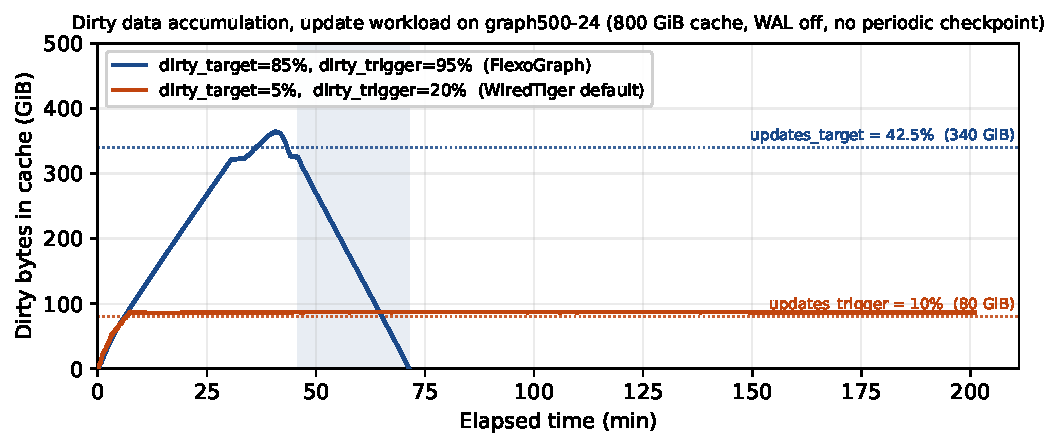
\includegraphics[width=\columnwidth]{fig/dynamic/dirty_accumulation.pdf}
  \caption{Dirty bytes resident in the WiredTiger cache during the graph500-24
  update workload, under \project{}'s eviction setting and under WiredTiger's
  defaults. Dotted lines mark the derived \texttt{updates} thresholds that
  actually bind. The shaded region is the interval in which a checkpoint is
  running. Under \project{}'s setting nothing is written to disk for the first
  31 minutes; under the defaults the dirty set is held flat at the
  application-thread trigger for the entire run.}
  \label{fig:dirty-accumulation}
\end{figure}

%%%%%%%%%%%%%%%%%%%%%%%%%%%%%%%%%%%%%%%%%%%%%%%%%%%%%%%%%%%%%%%%%%%%%%%%%%%%%%%%
\begin{figure}[t]
  \centering
  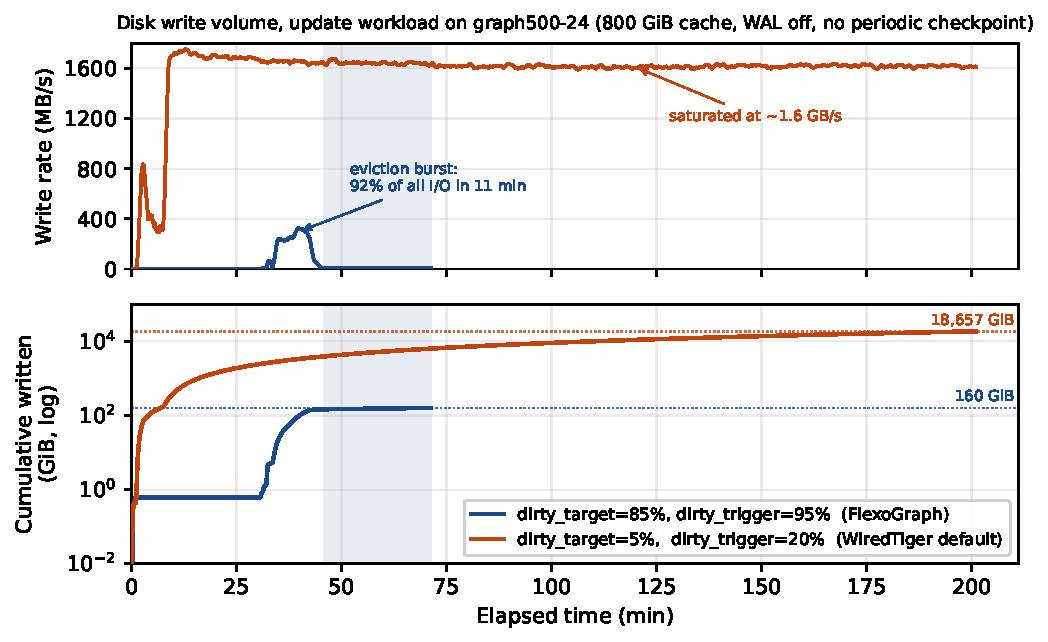
\includegraphics[width=\columnwidth]{fig/dynamic/write_volume.pdf}
  \caption{Disk traffic for the same two arms: instantaneous write rate (top)
  and cumulative volume (bottom, log scale; the arms differ by two orders of
  magnitude). \project{}'s setting writes nothing for 31~minutes and then
  performs 92\% of the run's I/O in an eleven-minute eviction burst; the
  default thresholds saturate write bandwidth at ${\sim}$1.6\,GB/s from
  minute~ten onward and never stop. Shaded regions mark a running checkpoint in the \project{} config.}
  \label{fig:write-volume}
\end{figure}
%%%%%%%%%%%%%%%%%%%%%%%%%%%%%%%%%%%%%%%%%%%%%%%%%%%%%%%%%%%%%%%%%%%%%%%%%%%%%%%%
%%%%%%%%%%%%%%%%%%%%%%%%%%%%%%%%%%%%%%%%%%%%%%%%%%%%%%%%%%%%%%%%%%%%%%%%%%%%%%%%

\autoref{fig:dirty-accumulation} plots the resident dirty set over time. The two
arms produce qualitatively different regimes.

\textbf{Under \project{}'s setting the run has three phases.} For the first
31~minutes the dirty set grows linearly to 322\,GiB and the block manager writes
\emph{nothing}: not a single page is evicted, because no threshold has been
crossed. 
The engine is, for this period, a pure in-memory store with a write-ahead structure that has never been written ahead.
At minute~30.7 the update byte count (322\,GiB inflated by the 8\% cache overhead, or 348\,GiB effective) crosses the derived \texttt{updates\_target} of 340\,GiB, and the eight background eviction threads begin working.
Eviction then peaks at 9{,}283~pages/s and 302\,MB/s, and in eleven minutes performs 92\% of all the disk writing the run will ever do.
The dirty set nevertheless continues to grow during this burst, to a peak of 364.3\,GiB, because the writers are still outrunning eviction.
Only when the update stream completes does the forced checkpoint drain the remaining 326\,GiB back to zero.
Throughout, application threads are never conscripted: the application-thread eviction wait is exactly zero and no page is evicted by a writer.

\textbf{Under WiredTiger's defaults the run has one phase.} The dirty set climbs to 87\,GiB within ten minutes (crossing the 80\,GiB derived \texttt{updates\_trigger}) and is then held flat there for the remainder of the run.
It is held flat by conscription: application threads perform 428.8~million page
evictions themselves and accumulate 768{,}192~thread-seconds of waiting for
cache, which is 88\% of all available writer thread-time.
Crucially, no checkpoint is running during any of this; eviction is entirely unobstructed.
The derived threshold alone is sufficient to spend the overwhelming majority of the write path's time on cache management rather than on graph updates.

The cost is visible in the disk traffic (\autoref{fig:write-volume}).
Write bandwidth saturates at ${\sim}$1.6\,GB/s within ten minutes and stays there: the writers are throttled to whatever the device will sustain. 
We stopped this arm after 201~minutes, at which point it had completed 61\% of the update log having written 18{,}657\,GiB (117$\times$ what \project{}'s setting wrote for the \emph{entire} workload, or ${\sim}$191$\times$ normalised per unit of work).

\textbf{The default configuration also degrades without bound.} Measured in
ten-minute windows, the cursor operation rate falls from 3{,}651\,K/s in the
first ten minutes to 431\,K/s in the second, an 8.5$\times$ collapse occurring
exactly as the dirty set crosses the 80\,GiB trigger.
It thereafter decays monotonically to 205\,K/s by minute~130, with no sign of a floor. 
Before the crossing this arm was in fact \emph{faster} than \project{}'s setting
(3{,}651\,K/s against 3{,}018\,K/s); the entire deficit is created at the
threshold.
We stopped the run because successive completion estimates kept receding (147, then 255, then 325~minutes) as the rate fell.

\autoref{tab:dirty-arms} summarises the two arms.

%%%%%%%%%%%%%%%%%%%%%%%%%%%%%%%%%%%%%%%%%%%%%%%%%%%%%%%%%%%%%%%%%%%%%%%%%%%%%%%%
\begin{table}[t]
  \centering
  \setlength{\tabcolsep}{5pt}\renewcommand{\arraystretch}{1.05}
  \small
  \begin{tabular}{l rr}
  \toprule
   & \project{} setting & WiredTiger default \\
  \midrule
  Fraction of update log completed & 100\%     & 61\% (stopped) \\
  Peak dirty bytes                & 364.3\,GiB & 87.7\,GiB \\
  Time to first disk write        & 31\,min    & ${<}$1\,min \\
  Bytes written to disk           & 160\,GiB   & 18{,}657\,GiB \\
  \dots{} of which by checkpoint  & 13\,GiB (8\%) & 0\,GiB \\
  Peak write bandwidth            & 327\,MB/s  & 1{,}754\,MB/s \\
  Pages evicted by writer threads & 0          & 428{,}817{,}961 \\
  Writer time waiting for cache   & 0\,s       & 768{,}192\,thread-s (88\%) \\
  Update throughput               & 1.010\,M~ops/s & see text \\
  \bottomrule
  \end{tabular}
  \caption{Update workload on graph500-24, SplitEdgeKey, 72 writers, WAL off,
  no periodic checkpoint. The two arms differ only in the four configured
  eviction thresholds. The default-threshold arm was stopped after
  201~minutes (2.8$\times$ the \emph{total} wall clock of the complete
  \project{} run), having finished 61\% of the update log; its throughput was
  still falling, so no single steady-state figure characterises it.}
  \label{tab:dirty-arms}
\end{table}
%%%%%%%%%%%%%%%%%%%%%%%%%%%%%%%%%%%%%%%%%%%%%%%%%%%%%%%%%%%%%%%%%%%%%%%%%%%%%%%%

\textbf{Takeaway.}
The configuration we adopt to make \project{} comparable with in-memory systems
postpones the cost of persistence and pays it in a single burst.
For 31~minutes the engine performs no I/O at all, and the reported throughput of 1.010\,M~ops/s is, in that window, an in-memory number.
That number is purchased by allowing 364\,GiB of unreconciled updates to accumulate (46\% of the configured cache), all of which must subsequently be reconciled and written.
WiredTiger's own defaults hold the dirty set to a quarter of that size, but spend 88\% of writer thread-time on cache eviction and write two orders of magnitude more data.
They never reach a steady state.
There is no setting of these thresholds that makes the work disappear: only a choice of when to pay and how violently.
This is the substance of the ``persistence machinery tax'' referred to in
\autoref{sec:eval:dynamic}: the in-memory baselines avoid the obligation to ever reconcile a page.
That reconciliation obligation, more than the I/O it produces, is what \project{} cannot escape while remaining persistable by construction.

\PM{The WiredTiger-default arm was stopped at 61\% of the update log rather than
run to completion; its counters are therefore lower bounds and it has no
end-to-end throughput figure. Both arms are $n{=}1$ and carry the 5\,s
statistics log, which perturbs absolute throughput; the numbers in
\autoref{fig:throughput-update} remain the uninstrumented ones.}
